\documentclass[12 pt]{article}
\usepackage{hyperref, fancyhdr, setspace, enumerate, amsmath,
  lastpage, amssymb, algpseudocode, bussproofs, tikz}
\usetikzlibrary{shapes.geometric}
\usetikzlibrary{positioning}
\EnableBpAbbreviations
\usepackage[margin=1 in]{geometry}
\allowdisplaybreaks
%\usepackage[dvipsnames]{xcolor}   %May be necessary if you want to color links
\hypersetup{
	%colorlinks=true, %set true if you want colored links
	linktoc=all,     %set to all if you want both sections and subsections linked
	linkcolor=black,  %choose some color if you want links to stand out
}
\usepackage{graphicx}
\graphicspath{{Images/}}
\author{Julian Lore}
\date{Last updated: \today}
\title{COMP 527: Logic and Computation}
\pagestyle{fancy}
\lhead{COMP 527}
\chead{\leftmark}
\rhead{Julian Lore}
\cfoot{Page \thepage \ of \pageref{LastPage}}
\newcommand{\tab}[1]{\hspace{.2\textwidth}\rlap{#1}}
\newenvironment{rcases}
  {\left.\begin{aligned}}
  {\end{aligned}\right\rbrace}
\begin{document}
	\onehalfspacing
	\maketitle
	\tableofcontents
    \section{01/08/19}
    \paragraph{Goal:}
    \begin{itemize}
    \item Introduction to the proof theoretic foundations
    \item Study the relationship to programming languages and their
      design
    \end{itemize}
    \paragraph{Schedule:}
    \begin{itemize}
    \item Week 1: Natural Deduction
    \item Week 2: Tutorial (Jacob) on using Tutch (proof assistant,
      program on writing Natural Deduction proofs)
    \item Week 3: Proofs in the natural deduction system and programs
      in the $\lambda$-calculus
    \item Week 4: First Order Logic
    \item Week 5: Induction (how we can add induction to logic,
      corresponds to recursion)
    \item Week 6/7: Programming with dependent types
    \item Week 8: Sequent calculus
    \item Week 9: Consistency
    \item Week 10: Proof search
    \item Week 11/12: Linear logic, modal logic or temporal logic
    \end{itemize}
    \subsection{Natural Deduction}
    \begin{itemize}
    \item G. Gentzen started describing it in the mid 30s
    \item Martin L\"of continued in the mid 80s
    \end{itemize}
    \paragraph{Motivation} To design a modular system for
    reasoning. Want to capture the reasoning of mathematicians (that's
    why it's called natural). It is modular because we define the
    meaning of each connective by themselves (will not refer to any
    other connective in the definition).
    \paragraph{Judgment} ``Something we know'' or ``something that is
    evident''
    \\ Ex. $A$ true, ``The proposition $A$ is true'' (Semantics)
    \\ $A$ wf, ``The proposition $A$ is syntactically well-formed''
    (Syntax)
    \\ $A$ true @ $t$, ``The proposition
    $A$ is true at time $t$''
    \\ Can describe both aspects (semantics and syntax) as judgment

    \paragraph{Example Grammar}
    Proposition $A, B:= T | \perp | A \land B | \ldots$
    \begin{prooftree}
      \AXC{}
      \UIC{T wf}
    \end{prooftree}
    \begin{prooftree}
      \AXC{}
      \UIC{$\perp$ wf}
    \end{prooftree}
    \begin{prooftree}
      \AXC{A wf}
      \AXC{B wf}
      \BIC{A $\land$ B wf}
    \end{prooftree}
    \begin{prooftree}
      \AXC{$J_1$ \ldots $J_n$}
      \UIC{$J$}
    \end{prooftree}
    $J_i$ are the premises, $J$ is the conclusion
    \\ $A$ true
    \begin{itemize}
    \item Introduction rules: How can we conclude $A$
    \item Elimination rules: What information can we extract from A?
      (i.e. T, $\perp$, $A \land B$, \ldots)
    \end{itemize}
    \begin{prooftree}
      \AXC{}
      \RL{T I (Introduction)}
      \UIC{T true}
    \end{prooftree}
    No elim rule for T
    \paragraph{Conjunction}
    \begin{prooftree}
      \AXC{A true}
      \AXC{B true}
      \RL{$\land$I}
      \BIC{$A \land B$ true}
    \end{prooftree}
    \begin{prooftree}
      \AXC{$A \land B$ true}
      \RL{$\land$E$_l$ (Elimination)}
      \UIC{$A$ true}
    \end{prooftree}
    \begin{prooftree}
      \AXC{$A \land B$ true}
      \RL{$\land$E$_r$}
      \UIC{$B$ true}
    \end{prooftree}
    What can we now prove?
    \begin{prooftree}
      \AXC{}
      \RL{$T$ I}
      \UIC{$T$ true}
      \AXC{}
      \RL{$T$ I}
      \UIC{$T$ true}
      \RL{$\land$ I}
      \BIC{$T \land T$ true}
    \end{prooftree}
    Is the following a proof?
    \begin{prooftree}
      \AXC{$A \land (B \land C)$ true}
      \RL{$\land$E$_r$}
      \UIC{$B \land C$ true}
      \RL{$\land$ E$_l$}
      \UIC{$B$ true}
    \end{prooftree}
    No, how do we know $A \land (B \land C)$ is true?

    Given the assumption (hypothesis) $A \land (B \land C)$ true, we
    can construct a proof for $B$ true (reasoning by
    assumption/hypothetical reasoning/derivation).
    \begin{prooftree}
      \AXC{}
      \RL{$u_1$}
      \UIC{$J_1$}
      \AXC{\ldots}
      \AXC{}
      \RL{$u_n$}
      \UIC{$J_n$}
      \TIC{\vdots}
      \noLine
      \UIC{$J$}
    \end{prooftree}
    \paragraph{Implication}
    \begin{prooftree}
      \AXC{}
      \RL{$u$}
      \UIC{$A$ true}
      \noLine
      \UIC{\vdots}
      \noLine
      \UIC{$B$ true}
      \RL{$ \supset$ I$^{u}$}
      \UIC{$A \supset B$ true}
    \end{prooftree}
    \begin{prooftree}
      \AXC{$A \supset B$ true}
      \AXC{$A$ true}
      \RL{$\supset$ E}
      \BIC{$B$ true}
    \end{prooftree}
    We do not include $A \supset B$ true, $B$ false, implies $A$
    false, because we did not add a judgment for false, only talking
    about things that are true. If we cannot say something is true, it
    is implied that it is false.

    Let's prove:
    \begin{prooftree}
      \AXC{}
      \RL{$u$}
      \UIC{$A$ true}
      \AXC{}
      \RL{$v$}
      \UIC{$B$ true}
      \RL{$\land$ I}
      \BIC{$A \land B$ true}
      \RL{$\supset I^v$}
      \UIC{$B \supset A \land B$ true}
      \RL{$\supset I^u$}
      \UIC{$A \supset (B\supset A \land B)$ true}
    \end{prooftree}
    \paragraph{Observations}
    \begin{enumerate}
    \item \underline{Order} of assumptions does not matter.
    \item Do I have to use an assumption? No. This is called \underline{weakening}.
      \\ Floating assumption that isn't used:
      \begin{prooftree}
        \AXC{}
        \RL{$v$}
        \UIC{$B$ true}
      \end{prooftree}
      \begin{prooftree}
        \AXC{}
        \RL{$u$}
        \UIC{$A$ true}
        \RL{$\supset I^v$}
        \UIC{$B\supset A$ true}
        \RL{$\supset I^u$}
        \UIC{$A \supset B \supset A$ true}
      \end{prooftree}
    \item Can we use assumptions more than once? Yes. This is called
      \underline{strengthening} (you contract multiple of these
      assumptions into one).
      \begin{prooftree}
        \AXC{}
        \RL{$u$}
        \UIC{$A$ true}
        \AXC{}
        \RL{$u$}
        \UIC{$A$ true}
        \RL{$\land$I}
        \BIC{$A \land A$ true}
        \RL{$\supset I^u$}
        \UIC{$A \supset (A \land A)$ true}
      \end{prooftree}
      This is a program that takes in an input and returns it twice.
    \end{enumerate}
    A simple proof:
    \begin{prooftree}
      \AXC{}
      \RL{$u$}
      \UIC{$A \land B$ true}
      \RL{$\land$ E$_l$}
      \UIC{$A$ true}
      \AXC{}
      \RL{$u$}
      \UIC{$A \land B$ true}
      \RL{$\land$ E$_r$}
      \UIC{$B$ true}
      \RL{$\land$I}
      \BIC{$B\land A$ true}
      \RL{$\supset I^u$}
      \UIC{$(A \land B) \supset (B \land A)$ true}
    \end{prooftree}
    \section{01/10/18}
    \subsection{Natural Deduction}
    \underline{A true}
    \paragraph{Conjunction}
    \begin{prooftree}
      \AXC{$A$ true}
      \AXC{$B$ true}
      \RL{$\land$ I}
      \BIC{$A \land B$ true}
    \end{prooftree}
    \begin{prooftree}
      \AXC{$A \land B$ true}
      \RL{$\land$E$_l$ (Elimination)}
      \UIC{$A$ true}
    \end{prooftree}
    \begin{prooftree}
      \AXC{$A \land B$ true}
      \RL{$\land$E$_r$}
      \UIC{$B$ true}
    \end{prooftree}
    \paragraph{Implications}
    This discharges the assumption $u$ and is the only rule we have
    right now that discharges assumptions.
    \begin{prooftree}
      \AXC{}
      \RL{$u$}
      \UIC{$A$ true}
      \noLine
      \UIC{\vdots}
      \noLine
      \UIC{$B$ true}
      \RL{$ \supset$ I$^{u}$}
      \UIC{$A \supset B$ true}
    \end{prooftree}
    \begin{prooftree}
      \AXC{$A \supset B$ true}
      \AXC{$A$ true}
      \RL{$\supset$ E}
      \BIC{$B$ true}
    \end{prooftree}
    \paragraph{Truth}
    \begin{prooftree}
      \AXC{}
      \RL{T I}
      \UIC{T true}
    \end{prooftree}
    To get the smallest complete example, we need to introduce
    $\perp$.
    \paragraph{Falsehood}
    No Intro-Rule for $\perp$.
    \begin{prooftree}
      \AXC{$\perp$ true}
      \RL{$\perp$ E}
      \UIC{$A$ true}
    \end{prooftree}
    Define Negation as an abbreviation (notational definition)
    $$\neg A \equiv A \supset \perp$$
    \begin{prooftree}
      \AXC{}
      \RL{u}
      \UIC{$A \land \neg A$}
      \RL{$\land$ E$_l$}
      \UIC{$A$}
      \AXC{}
      \RL{u}
      \UIC{$A \land \neg A$}
      \RL{$\land$ E$_r$}
      \UIC{$\neg A \equiv (A \supset \perp)$}
      \RL{$\supset$ E}
      \BIC{$\perp$}
      \RL{$\supset$ I$^u$}
      \UIC{$\neg (A \land \neg A)$ true}
    \end{prooftree}
    If we could prove $\perp$ from no assumptions, then our system
    would be inconsistent.
    \paragraph{Examples}
    \begin{prooftree}
      \AXC{}
      \RL{u}
      \UIC{$A\supset (B \land C)$ true}
      \AXC{}
      \RL{v}
      \UIC{$A$ true}
      \RL{$\supset$ E}
      \BIC{$B \land C$ true}
      \RL{$\land$ E$_l$}
      \UIC{$B$ true}
      \RL{$\supset$I$^v$}
      \UIC{$A \supset B$ true}
      \AXC{}
      \RL{u}
      \UIC{$A \supset (B \land C)$ true}
      \AXC{}
      \RL{v}
      \UIC{$A$ true}
      \BIC{$B \land C$}
      \RL{$\land$ E}
      \UIC{$C$ true}
      \RL{$\supset$ I$^v$}
      \UIC{$A \supset C$ true}
      \RL{$\land$ I}
      \BIC{$(A \supset B) \land (A \supset C)$ true}
      \RL{$\supset$ I$^u$}
      \UIC{$(A \supset (B \land C)) \supset ((A \supset B) \land
        (A \supset C)) = (A \land \neg A) \supset \perp$ true}
    \end{prooftree}
    Note that the assumptions u and v are used twice, but in different
    areas.
    \begin{prooftree}
      \AXC{}
      \RL{u}
      \UIC{$A$}
      \AXC{}
      \RL{v}
      \UIC{$\neg A$}
      \RL{$\supset$ E}
      \BIC{$\perp$}
      \RL{$\supset$ I$^v$}
      \UIC{$\neg \neg A = \neg A \supset \perp$ true}
      \RL{$\supset$ I$^u$}
      \UIC{$A \supset \neg \neg A$ true}
    \end{prooftree}
    Is $A = \neg \neg A$? We cannot prove this in this logic unless we
    assume an axiom (although it is true for classical logic).

    For a proof, we must discharge all assumptions we make.

    \paragraph{Local Soundness}
    How do we know the rules we defined for natural deduction make
    sense?

    Elimination Rules are not too strong (they don't allow us to
    conclude more than we should be able to). If the rules are too
    strong, we'll be able to prove things that we shouldn't be able
    to, more than we had to start with.

    Given a proof $\delta$ for $A$ true and a proof $\varepsilon$ for
    $B$ true, we can prove $A$ true.
    \begin{center}
      \AXC{$\delta$}
      \noLine
      \UIC{$A$ true}
      \AXC{$\varepsilon$}
      \noLine
      \UIC{$B$ true}
      \RL{$\land$ I}
      \BIC{$A \land B$ true}
      \RL{$\land$ E}
      \UIC{$A$ true}
      \DP
      \begin{tabular}{c}
      $\delta$
      \\ $\Longrightarrow A$ true
      \end{tabular}
    \end{center}
    \begin{center}
      \AXC{$\delta$}
      \noLine
      \UIC{$A$ true}
      \AXC{$\varepsilon$}
      \noLine
      \UIC{$B$ true}
      \RL{$\land$ I}
      \BIC{$A \land B$ true}
      \RL{$\land$ E}
      \UIC{$B$ true}
      \DP
    \begin{tabular}{c}
      $\varepsilon$\\ $\Longrightarrow B$ true
    \end{tabular}
    \end{center}
    \paragraph{Local Completeness}
    Elimination Rules are not too weak, i.e. we are expanding proofs.
    \begin{center}
    \begin{tabular}{c}
      $\delta$ \\ $A \land B$ true $\Longrightarrow$
    \end{tabular}
    \AXC{$\delta$}
    \noLine
    \UIC{$A \land B$ true}
    \RL{$\land$ E$_l$}
    \UIC{$A$ true}
    \AXC{$\delta$}
    \noLine
    \UIC{$A \land B$ true}
    \RL{$\land$ E$_r$}
    \UIC{$B$ true}
    \RL{$\land$ I}
    \BIC{$A \land B$ true}
    \DP
    \end{center}
    \paragraph{Local Soundness (Implication)}
    \begin{center}
    \AXC{}
      \RL{u}
      \UIC{$A$ true}
      \noLine
      \UIC{\vdots}
      \noLine
      \UIC{$\delta^u$}
      \noLine
      \UIC{$B$ true}
      \RL{$\supset$ I$^u$}
      \UIC{$A \supset B$ true}
      \AXC{$\varepsilon$}
      \noLine
      \UIC{$A$ true}
      \RL{$\supset$ E}
      \BIC{$B$ true}
      \DP
      \begin{tabular}{c}
        $\varepsilon$
        \\$A$ true
      \\$[\varepsilon/u] (\delta)$
      \\$\Longrightarrow B$ true 
      \end{tabular}
    \end{center}
    \paragraph{Substitution Principle}
    \begin{center}
    If
      \AXC{}
      \RL{u}
      \UIC{$A$ true}
      \noLine
      \UIC{$\vdots$}
      \noLine
      \UIC{$\delta$}
      \noLine
      \UIC{$B$ true}
      \DP
      and
      \begin{tabular}{c}
        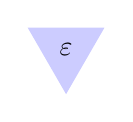
\begin{tikzpicture} [
          triangle/.style = {fill=blue!20, regular polygon, regular polygon sides=3 },
          node rotated/.style = {rotate=180},
          border rotated/.style = {shape border rotate=180}
          ]
          \node[triangle, border rotated] {$\varepsilon$};
        \end{tikzpicture}\\
        $A$ true 
      \end{tabular},
      then
      \begin{tabular}{c}
        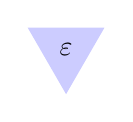
\begin{tikzpicture} [
          triangle/.style = {fill=blue!20, regular polygon, regular polygon sides=3 },
          node rotated/.style = {rotate=180},
          border rotated/.style = {shape border rotate=180}
          ]
          \node[triangle, border rotated] {$\varepsilon$};
        \end{tikzpicture}\\
    $A$ true \\ $\delta$ \\ $B$ true
      \end{tabular}
    \end{center}

    Basically, if we have a proof for $A$ true and from $A$ true we
    can show $B$ true, then we have a proof for $B$ true.

    \paragraph{Local Completeness}
    \begin{center}
      \AXC{$\alpha$}
      \noLine
      \UIC{$A \supset B$ true}
      \AXC{}
      \RL{u}
      \UIC{$A$ true}
      \RL{$\supset$ E}
      \BIC{$B$ true}
      \RL{$\supset$ I$^u$}
      \UIC{$A \supset B$ true}
      \DP
      \begin{tabular}{c}
        $\alpha$
        \\$\Longrightarrow A \supset B$ true
      \end{tabular}
    \end{center}
    So we can prove $A \supset B$ from $A \supset B$.

    Another form of $\land$ elimination:
    \begin{prooftree}
      \AXC{$A \land B$ true}
      \AXC{}
      \RL{u}
      \UIC{$A$ true}
      \AXC{}
      \RL{v}
      \UIC{$B$ true}
      \noLine
      \BIC{\vdots}
      \noLine
      \UIC{$C$ true}
      \RL{$\land E^{u,v}$}
      \BIC{$C$ true}
    \end{prooftree}
    We could use this new rule and check for local soundness and
    completeness like above.

    Could have unused, floating assumption:
    \begin{prooftree}
      \AXC{}
      \RL{a}
      \UIC{$A$ true}
    \end{prooftree}
    \begin{prooftree}
      \AXC{}
      \RL{u}
      \UIC{$A \land B$}
      \RL{b}
      \UIC{$B$ true}
      \AXC{\vdots}
      \noLine
      \UIC{$A$ true}
      \BIC{$B \land A$ true}
      \RL{$\supset$ I$^u$}
      \UIC{$A \land B \supset B \land A$ true}
    \end{prooftree}
    \subsection{Disjunction}
    Intro-Rules:
    \begin{prooftree}
      \AXC{$A$ true}
      \RL{$\lor$ I$_l$}
      \UIC{$A \lor B$ true}
    \end{prooftree}
    \begin{prooftree}
      \AXC{$B$ true}
      \RL{$\lor$ I$_r$}
      \UIC{$A \lor B$ true}
    \end{prooftree}
    Might be tempted to make the following rule:
    \begin{prooftree}
      \AXC{$B$ true}
      \RL{$\lor$ I$_r$}
      \UIC{$A \lor B$ true}
      \RL{?}
      \UIC{$A$ true}
    \end{prooftree}
    This is locally unsound! Got information we didn't start with.

    We also cannot introduce:
    \begin{prooftree}
      \AXC{$A \lor B$}
      \UIC{$\neg A \supset B$ true}
    \end{prooftree}
    This violates our principle of modularity, as we don't want to
    refer to a different kind of connective.

    Our elimination rule:
    \begin{prooftree}
      \AXC{$A \lor B$ true}
      \AXC{}
      \RL{u}
      \UIC{$A$ true}
      \noLine
      \UIC{\vdots}
      \noLine
      \UIC{$C$ true}
      \AXC{}
      \RL{v}
      \UIC{$B$ true}
      \noLine
      \UIC{\vdots}
      \noLine
      \UIC{$C$ true}
      \RL{$\lor$ E}
      \TIC{$C$ true}
    \end{prooftree}
    \paragraph{Example}
    \begin{prooftree}
      \AXC{}
      \RL{u}
      \UIC{$A \lor (B \land C)$ true}
      \AXC{}
      \RL{a}
      \UIC{$A$ true}
      \RL{$\lor$ I$_l$}
      \UIC{$A \lor C$ true}
      \AXC{}
      \RL{b}
      \UIC{$B \land C$ true}
      \RL{$\land$ E$_l$}
      \UIC{$A \lor B$ true}
      \UIC{$B$ true}
      \RL{$\lor$ I$_r$}
      \RL{$\lor$ E}
      \TIC{$A \lor B$ true}
      \AXC{\vdots}
      \noLine
      \UIC{$A \lor C$ true} % Same proof as other thing (almost)
      \RL{$\lor$ I}
      \BIC{$(A \lor B)\land (A \lor C)$}
      \RL{$\supset$ I}
      \UIC{$(A \lor (B \land C))\supset (A \lor B)\land (A \lor C)$}
    \end{prooftree}
\end{document}